\documentclass[12pt, a4paper]{article}
\usepackage[utf8]{inputenc}
\usepackage[brazilian]{babel} % Hifenização e dicionário
\usepackage[left=3.00cm, right=2.00cm, top=3.00cm, bottom=2.00cm]{geometry}
\usepackage{enumitem} % Para itemsep etc
\usepackage{longtable} % Dependência do longtabu
\usepackage{tabu} % Para melhor criação de tabelas
\usepackage{zi4} % Para fonte de códigos
\usepackage{listings} % Para códigos
\usepackage{lstautogobble} % Códigos indentados corretamente
\usepackage{color} % Para coloração de códigos
\usepackage{mathpazo} % Palatino
\usepackage{parskip} % Linha em branco entre parágrafos em vez de recuo
\usepackage{graphicx}
\usepackage{verbatim} % Para comentários
\usepackage{booktabs}
\usepackage{amsmath} % bmod
\usepackage[breaklinks]{hyperref}

\DeclareGraphicsExtensions{.pdf,.png}

\newcommand{\code}[1]{{\lstinline{#1}}}

\usepackage{listings}
\lstset{
    autogobble,
    columns=fullflexible,
    showspaces=false,
    showtabs=false,
    breaklines=true,
    showstringspaces=false,
    breakatwhitespace=true,
    escapeinside={(*@}{@*)},
    basicstyle=\ttfamily\footnotesize,
    frame=l,
    framesep=12pt,
    xleftmargin=12pt,
    tabsize=4,
    captionpos=b
}

\begin{document}
\begin{center}
    \textsc{Universidade Federal do Rio Grande do Norte} \\
    \textsc{Departamento de Informática e Matemática Aplicada}
\end{center}

\bigskip

\begin{tabular}{@{}ll@{}}
    \emph{Disciplina:} & DIM0612 --- Programação Concorrente \\
    \emph{Docente:}    & Everton Ranielly de Sousa Cavalcante \\
    \emph{Discente:}   & Felipe Cortez de Sá \\
\end{tabular}

\bigskip

\begin{center}
\large Multiplicação de matrizes
\end{center}

\bigskip

\section{Introdução}
Este relatório descreve a implementação de algoritmos para multiplicação de
matrizes de forma sequencial e concorrente utilizando múltiplas threads,
detalhando as estratégias utilizadas e comparando resultados obtidos a fim de
verificar se a adaptação concorrente gera ganho de desempenho.

\section{Detalhes da implementação}
O problema foi resolvido utilizando a linguagem de programação C++11 com a
biblioteca \code{std::thread}. As matrizes $ A $, $ B $ e $ C $ foram
codificadas como vetores unidimensionais (arrays estilo C) de tamanho $ n^2 $,
aproveitando o fato de que as matrizes de entrada e saída são quadradas.
Terminada a multiplicação entre matrizes, o resultado é salvo em um arquivo
\code{Cnxn.txt}, onde \code{n} é o valor de entrada do programa.

Na implementação com $ t $ \emph{threads}, cada thread é responsável pelo
cálculo de $ \frac{n^2}{t} $ elementos da matriz $ C $. Caso a divisão não seja
exata, a última thread calcula o resto da divisão, ou seja, $ \frac{n^2}{t} +
\left[ n^2 \pmod t \right] $ elementos. As threads são criadas na chamada do
método \code{emplace\_back}, que inicializa as threads da função
\code{multThread} com seus parâmetros, incluindo os índices do primeiro e
último elementos da matriz $ C $ que devem ser calculados pela \emph{thread}.

\begin{figure}[h]
\centering
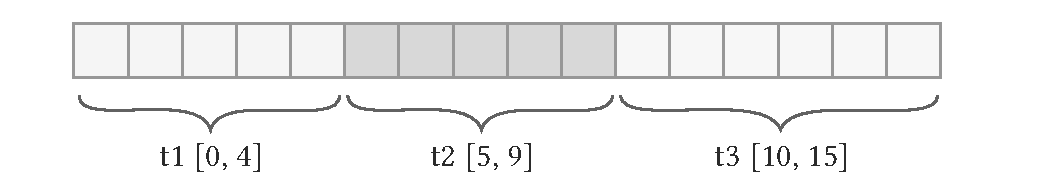
\includegraphics[width=.7\textwidth]{diagram_1}
\label{fig:f1}
\caption{Matriz $ C $ $ 4x4 $ com três threads}
\end{figure}

Foi selecionado o compilador \code{clang} com a flag \code{-O3} para
otimizações. O Makefile também funciona para distribuições Linux, utilizando o
compilador \code{g++} e a flag \code{-pthread}.

\subsection{Medição de desempenho}
Foi utilizada a biblioteca \code{std::chrono} para medir o tempo de execução.
Na implementação sequencial, o \emph{timer} inicia antes dos laços de
multiplicação e para depois dos laços. Na implementação com \emph{threads}, o
\emph{timer} inicia no momento anterior à criação da primeira \emph{thread} e
para após o último \code{join()}, isto é, quando todas as threads concluíram
sua execução. A precisão do timer é de nanossegundos, convertidos para
milissegundos para facilitar a visualização.

\subsection{Testes}
Os testes foram realizados em um MacBook Pro com sistema operacional Mac OS X El
Capitan (10.11.6), processador Intel Core i5, 2.5GHz com dois núcleos e memória
RAM de 8GB.

Os testes foram automatizados com um script programado em \emph{Python} que
executa os programas sequencial e concorrente com 20 repetições para cada
\emph{workload}. No final da execução, os valores mínimo, médio, máximo e
desvio padrão de cada teste são escritos (concatenados) no arquivo
\code{resultado.txt} para futura referência.

Como a multiplicação de duas matrizes $ 2048 \times 2048 $ leva um tempo
considerável, não seria viável realizar todos os testes para múltiplos tamanhos
de \emph{threads}. Foram calculados, então, tempos de execução para a
multiplicação de matrizes $ 512 \times 512 $ com quantidades de \emph{thread}
diferentes. Como pode ser visto na figura \ref{fig:f2}, após o ganho inicial de
desempenho não há variação considerável no tempo de execução ao aumentar o
número de \emph{threads}. Os testes concorrentes foram feitos com quatro \emph{threads}.

\begin{figure}[!h]
\centering
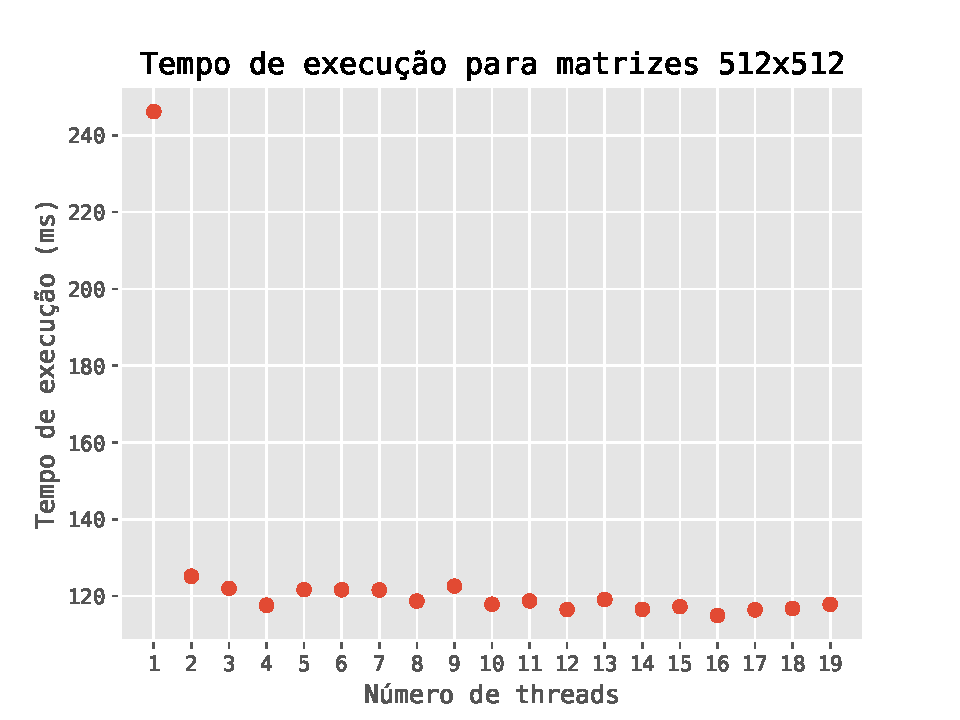
\includegraphics[width=.7\textwidth]{512_20threads}
\label{fig:f2}
\caption{Tempos de execução médios para quantidades de threads diferentes}
\end{figure}

\section{Resultados}
A tabela \ref{table1} mostra os tempos de execução registrados nos testes
realizados.  Observa-se que as soluções sequenciais apresentam desempenho
melhor para \emph{workloads} menores, e há ganho de desempenho (\emph{speedup}
$ > 1 $) apenas a partir do caso de matrizes com $ 128^2 $ elementos. Para
matrizes maiores, o \emph{speedup} é aproximadamente 2, ou seja, a solução
concorrente é duas vezes mais eficiente que a sequencial.

\begin{table}[!h]\footnotesize
    \centering
    \scalebox{0.8}{
        \begin{tabular}{ c c c c c c c c c c }
            \toprule
            \multicolumn{1}{r}{} & \multicolumn{4}{c}{Sequencial} & \multicolumn{4}{c}{4 threads} \\
            \cmidrule(r){2-5} \cmidrule(r){6-9}
            Carga & min    & med     & max    & $ \sigma $    & min & med & max & $ \sigma $ & \emph{speedup} \\
            \hline
            $ 4    ^2 $ & 0.0004 & 0.0018  & 0.0038 & 0.0011   & 0.1642 & 0.2129 & 0.3101 & 0.0365 & 0.0084 \\
            $ 8    ^2 $ & 0.0008 & 0.0032  & 0.0055 & 0.0014   & 0.1604 & 0.2912 & 1.8631 & 0.3624 & 0.1098 \\
            $ 16   ^2 $ & 0.0038 & 0.0074  & 0.0186 & 0.0031   & 0.1862 & 0.6439 & 3.6419 & 0.9205 & 0.0114 \\
            $ 32   ^2 $ & 0.0226 & 0.0369  & 0.0692 & 0.0117   & 0.1990 & 1.2316 & 8.9507 & 2.1793 & 0.0299 \\
            $ 64   ^2 $ & 0.1718 & 0.2762  & 0.3729 & 0.0576   & 0.3179 & 0.5539 & 1.4585 & 0.3039 & 0.4986 \\
            $ 128  ^2 $ & 2.0335 & 2.4222  & 3.3182 & 0.3979   & 1.3423 & 1.9905 & 4.4010 & 0.6620 & 1.2168 \\
            $ 256  ^2 $ & 17.7653 & 23.2958 & 32.1696 & 4.0813   & 8.9444 & 12.8657 & 17.0312 & 2.0607 & 1.8106 \\
            $ 512  ^2 $ & 225.0580 & 259.6764  & 357.5310 & 31.3413   & 114.7560 & 125.2099 & 138.2650 & 6.6438 & 2.0739 \\
            $ 1024 ^2 $ & 9818.3900 & 10020.0315  & 10819.9000 & 246.6014   & 5098.48 & 5196.9255 & 5307.7500 & 56.8640 & 1.9280 \\
            $ 2048 ^2 $ & 86893.0000 & 88398.8450  & 96279.5000 & 2342.1524   & 44313.3000 & 44531.8250 & 44983.4000 & 170.0722 & 1.9850 \\
            \bottomrule
        \end{tabular}
    }
    \label{table1}
    \caption{Tempos de execução em milissegundos}
\end{table}

\begin{figure}[h]
\centering
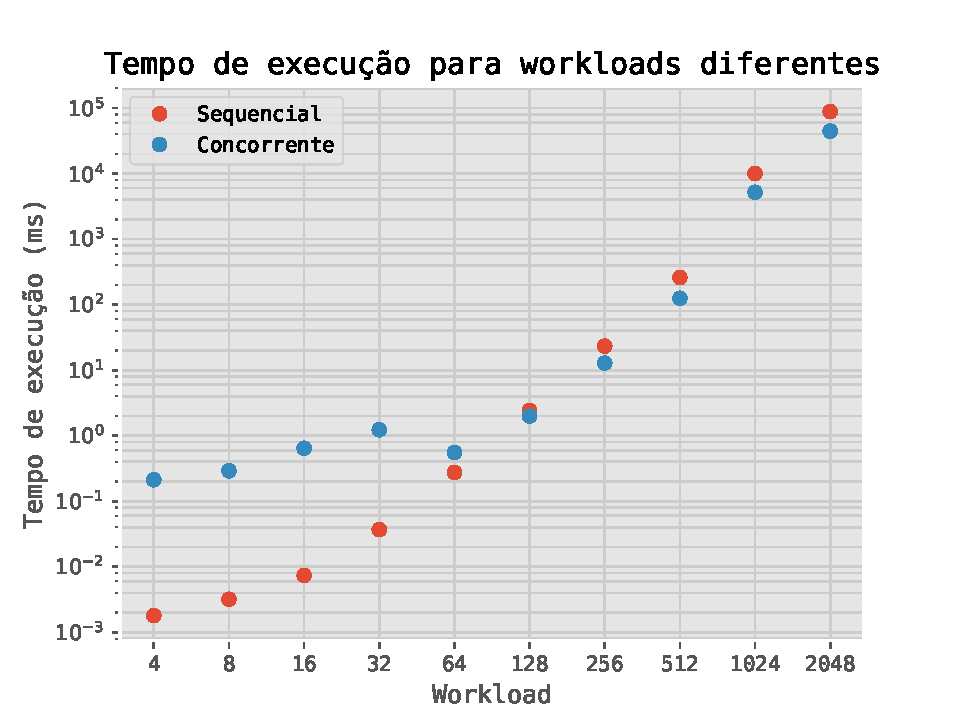
\includegraphics[width=.7\textwidth]{times}
\label{fig:f2}
\end{figure}

\section{Discussão}
A partir da realização desse trabalho foi possível concluir que o uso de
\emph{threads} pode aumentar o desempenho na resolução de problemas paralelos.
É interessante observar que utilizar múltiplas \emph{threads} pode aumentar o
tempo de execução para cargas menores.  Para trabalhos futuros, seria
interessante verificar como mais núcleos no processador podem aumentar o
desempenho e quantificar a melhoria.

\end{document}
